\documentclass[french]{standalone}
\usepackage{babel}
\usepackage{tkz-fct}
\usepackage{tkz-euclide}
\usepackage{color}
\usepackage{numprint}

\renewcommand*\familydefault{\sfdefault}
\usepackage{sansmath}
\sansmath
\definecolor{gray75}{gray}{0.75}

\begin{document}
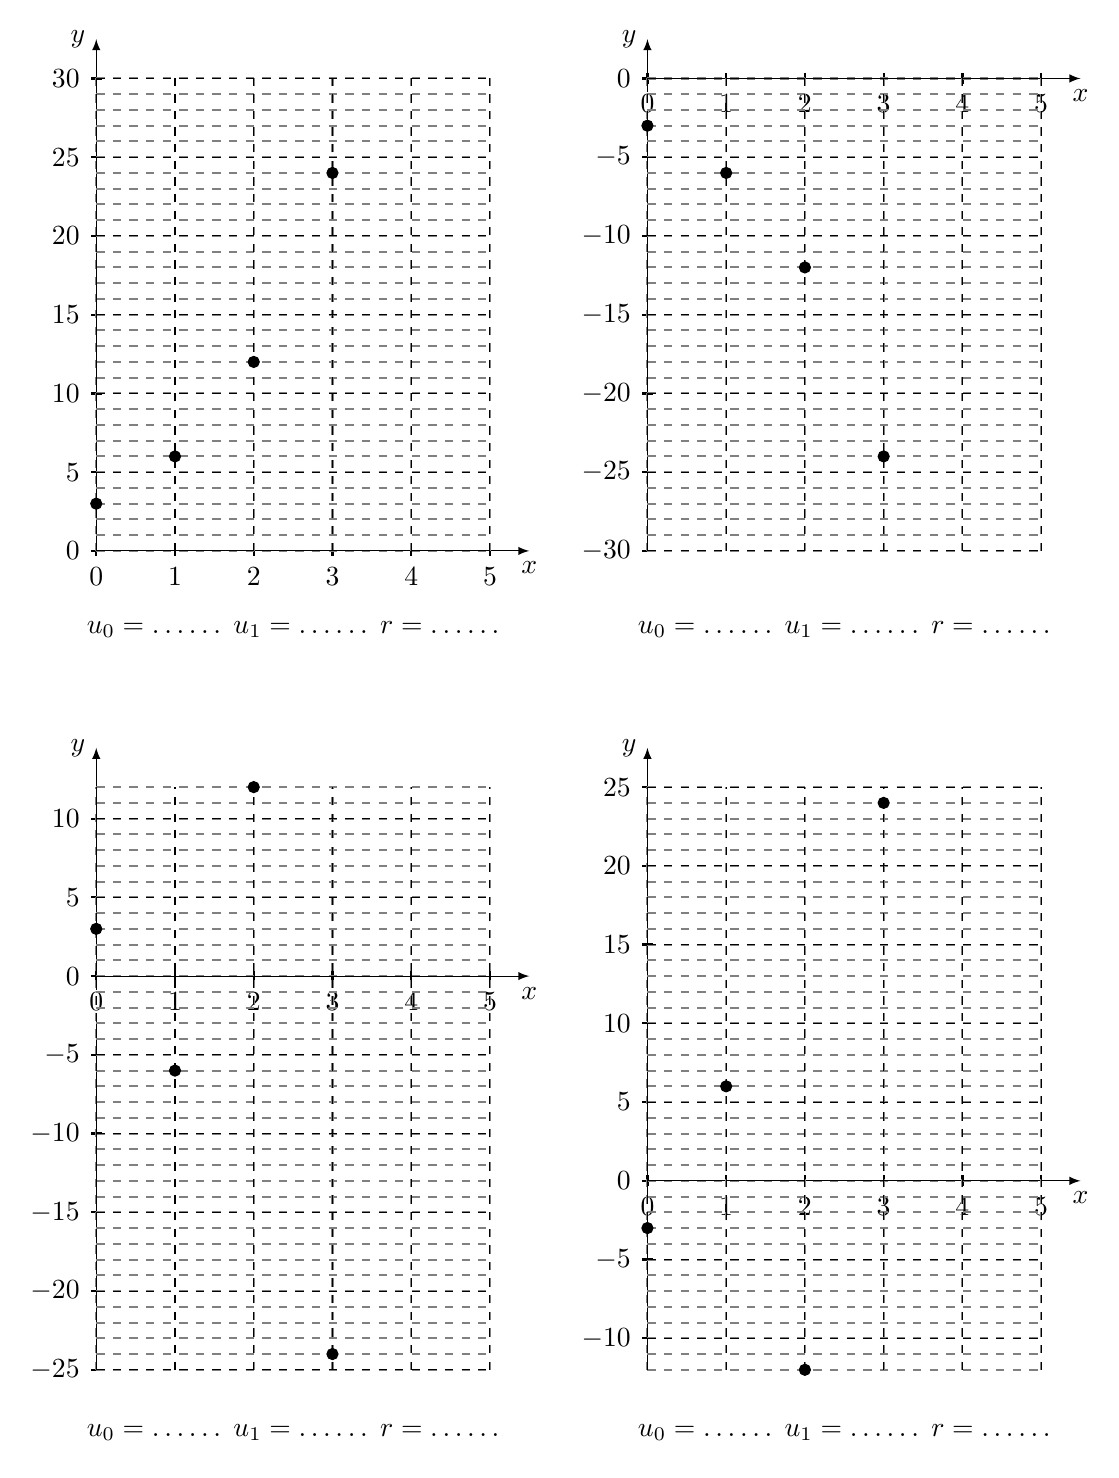
\begin{tikzpicture}
\tkzInit[xmin=0,xmax=5,ymin=0,ymax=30, ystep=5]
\tkzAxeXY
   \begin{scope}[dashed]
     \tkzGrid[color=black, sub, subxstep=1, subystep=1]
   \end{scope}
\tkzSetUpPoint[size = 4]
\global\edef\tkzFctLast{(3*exp(ln(2)*x))}
\foreach \va in {0,...,3}{%
  \tkzDefPointByFct[draw](\va)
}
\tkzText(2.5,-5){$u_{0}=\ldots\ldots\; u_{1}=\ldots\ldots\; r=\ldots\ldots$}
\begin{scope}[xshift=7cm, yshift=6cm]
 \tkzInit[xmin=0,xmax=5,ymin=-30,ymax=0, ystep=5]
\tkzAxeXY
   \begin{scope}[dashed]
     \tkzGrid[color=black, sub, subxstep=1, subystep=1]
   \end{scope}
\tkzSetUpPoint[size = 4]
\global\edef\tkzFctLast{(-3*exp(ln(2)*x))}
\foreach \va in {0,...,3}{%
  \tkzDefPointByFct[draw](\va)
}
\tkzText(2.5,-35){$u_{0}=\ldots\ldots\; u_{1}=\ldots\ldots\; r=\ldots\ldots$}

\end{scope}
\begin{scope}[xshift=7cm, yshift=-8cm]
 \tkzInit[xmin=0,xmax=5,ymin=-12,ymax=25, ystep=5]
\tkzAxeXY
   \begin{scope}[dashed]
     \tkzGrid[color=black, sub, subxstep=1, subystep=1]
   \end{scope}
\tkzSetUpPoint[size = 4]
\global\edef\tkzFctLast{(-3*exp(ln(2)*x))}
\foreach \va in {0,2}{%
  \tkzDefPointByFct[draw](\va)
}
\global\edef\tkzFctLast{(3*exp(ln(2)*x))}
\foreach \va in {1,3}{%
  \tkzDefPointByFct[draw](\va)
}
\tkzText(2.5,-16){$u_{0}=\ldots\ldots\; u_{1}=\ldots\ldots\; r=\ldots\ldots$}

\end{scope}
\begin{scope}[xshift=0cm, yshift=-5.4cm]
 \tkzInit[xmin=0,xmax=5,ymin=-25,ymax=12, ystep=5]
\tkzAxeXY
   \begin{scope}[dashed]
     \tkzGrid[color=black, sub, subxstep=1, subystep=1]
   \end{scope}
\tkzSetUpPoint[size = 4]
\global\edef\tkzFctLast{(3*exp(ln(2)*x))}
\foreach \va in {0,2}{%
  \tkzDefPointByFct[draw](\va)
}
\global\edef\tkzFctLast{(-3*exp(ln(2)*x))}
\foreach \va in {1,3}{%
  \tkzDefPointByFct[draw](\va)
}
\tkzText(2.5,-29){$u_{0}=\ldots\ldots\; u_{1}=\ldots\ldots\; r=\ldots\ldots$}

\end{scope}
\end{tikzpicture}
\end{document}
